\chapter{Modélisation}
\section{Modéle 1: Long Short-Term Memory (LSTM)}
\subsection{Définition}
Long Short-Term Memory (LSTM) est un type spécial de réseau de neurones. Il a été créé pour pallier les faiblesses des réseaux de neurones récurrents (RNN) standards, comme le souci des gradients qui s’estompent. Les LSTM, à la différence des RNN simples, apprennent mieux les liens à long terme. Ils sont super utiles pour comprendre le langage humain et prévoir les événements futurs.
\subsection{Architecture}
L’architecture des LSTMs se base sur un principe clé : les cellules LSTM. Ces cellules gèrent le flux d’informations au moyen de trois portes de la mémoire LSTM importantes. On a la porte d’oubli, la porte d’entrée et la porte de sortie. Les fonctions d’activation sigmoïdales permettent à ces portes de fonctionner de manière optimale.
\\
\\
Ces composantes LSTM jouent un rôle crucial. Elles préservent les informations essentielles sur le long terme. En même temps, elles préviennent les problèmes de gradient explosif ou disparu.
\\
\\
• Porte d’oubli: Décide des informations à garder ou à effacer. Un score près de 0 signifie oublier, près de 1 signifie conserver.
\\
• Porte d’entrée: Juge l’importance des nouvelles informations. Une note près de 0 indique peu d’importance, proche de 1 indique beaucoup d’importance.
\\
• Porte de sortie: Gère combien d’informations vont vers l’état caché suivant. oₜ proche de 0, peu transmis ; proche de 1, beaucoup est transmis.
\\
\\
Grâce à cette structure avancée, l’architecture des LSTMs surpasse les limites des RNN traditionnels. Cela concerne surtout la gestion des dépendances à long terme. Les cellules LSTM et leurs portes complexes aident à relever divers défis.
\begin{figure}[h!]
    \centering
    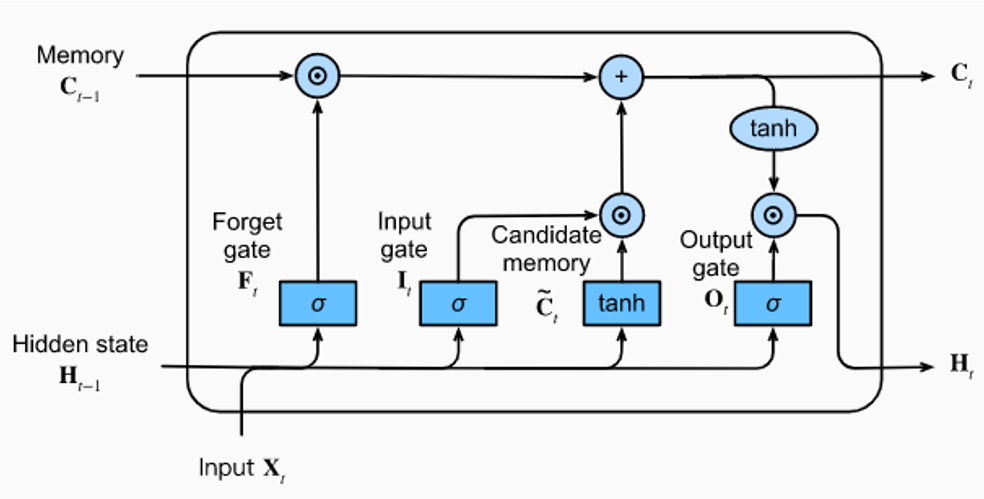
\includegraphics[width=1\textwidth]{124.png}
    \caption{Architecture du modéle LSTM}
    \label{fig:conf_matrix}
\end{figure}
\\
\\
\subsection{Fonctionnement}
Le fonctionnement d’une cellule LSTM se déroule en plusieurs étapes :
\\
\\
• Décider quoi oublier : La porte d’oubli analyse l’état précédent \( C_{t-1} \) et l’entrée actuelle \( x_t \) pour éliminer les informations inutiles.
\\
• La porte d’entrée et la mémoire candidate déterminent quelles nouvelles informations doivent être ajoutées à l’état de cellule.
\\
• Mettre à jour l’état de cellule : \[
C_t = f_t \ast C_{t-1} + i_t \ast \tilde{C}_t
\]

\noindent
⮕ Combinaison des informations conservées et des nouvelles informations.
\\
• Produire la sortie : \[
h_t = o_t \ast \tanh(C_t)
\]

\noindent
⮕ L’état de cellule filtré par la porte de sortie devient la sortie de la cellule.
\subsection{Compositions}
Le modèle LSTMClassifier est construit en héritant de la classe nn.Module de PyTorch. Il est composé de plusieurs couches :
\\
\\
• Embedding Layer : Transforme les mots d’entrée (représentés par des indices) en vecteurs denses de taille fixe (embedding dim = 100), et Chaque mot unique du vocabulaire (vocab size = 30522) a son propre vecteur.
\\
• LSTM Layer : 
\\
Cœur du modèle, capable d’apprendre les dépendances à long terme dans le texte.
\\
La dimension de sortie de chaque LSTM unit est dimension = 32.
\\
La couche LSTM est composée de 32 unités avec 1 couche.
\\
• Dropout Layer : Permet de régulariser le modèle et de réduire le surapprentissage en désactivant aléatoirement 50\% des neurones à chaque étape.
\\
• Fully Connected Layer : Une couche linéaire qui transforme la sortie du LSTM en une valeur unique, ensuite passée à une fonction sigmoïde pour obtenir une probabilité comprise entre 0 et 1.
\section{Modéle 2 : Convolutional Neural Network (CNN)}
\subsection{Définition}
Les Convolutional Neural Networks, ou CNN, sont une classe de réseaux de neurones utilisés dans le Deep Learning ou l'apprentissage profond, particulièrement efficaces pour analyser des données visuelles telles que des images et des vidéos. Cependant, ils se révèlent également très performants pour le traitement du texte, car leurs filtres convolutifs permettent de détecter des motifs locaux dans les séquences de mots, similaires à la manière dont ils identifient des formes dans une image.
\subsection{Architecture}
\begin{figure}[h!]
    \centering
    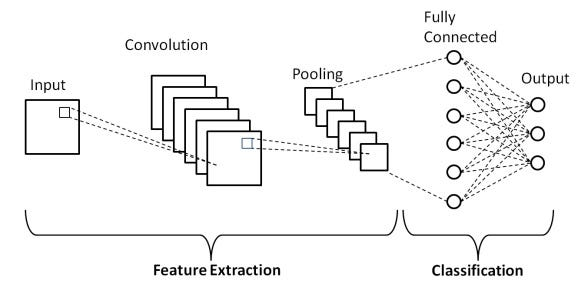
\includegraphics[width=1\textwidth]{15.jpg}
    \caption{Architecture du modéle CNN}
    \label{fig:conf_matrix}
\end{figure}
\\
Le modèle CNNClassifier hérite de nn.Module de PyTorch et est composé des couches suivantes :
\\
\\
• Embedding Layer : Transforme chaque mot d’entrée en un vecteur dense de taille embedding\_dim = 300. et Les tokens de padding sont mappés à des vecteurs nuls (pad\_idx).
\\
• Convolutional Layers (1D) : Plusieurs couches de convolution appliquent des filtres de tailles différentes (filter\_sizes = [3,4,5]) sur les embeddings, Chaque filtre détecte un motif spécifique dans le texte et Le nombre de filtres varie selon la taille (num\_filters = [100,200,300]).
\\
• Activation ReLU : Introduit la non-linéarité après chaque convolution pour permettre au modèle d’apprendre des motifs complexes.
\\
• Max Pooling : Réduit la dimension des cartes de caractéristiques tout en conservant les informations les plus importantes (valeurs maximales).
\\
• Fully Connected Layer : La sortie des différentes convolutions est concaténée puis passée dans une couche linéaire et Produit un score pour la classification binaire.
\\
• Dropout : Permet de régulariser le modèle en supprimant aléatoirement 50\% des neurones avant la couche fully connected.
\\
• Sigmoid Activation : Convertit le score en probabilité entre 0 et 1 pour prédire la classe positive ou négative.
\subsection{Fonctionnement}
Le fonctionnement d’un réseau de neurones convolutif (CNN) se déroule en plusieurs étapes :
\\
\\
• Appliquer la convolution : La couche de convolution analyse l’image d’entrée \(X\) à l’aide d’un filtre \(K\) afin d’extraire des caractéristiques locales comme les bords ou les textures.
\\
• Calculer la carte de caractéristiques : Le filtre se déplace sur l’image et calcule le produit de convolution pour chaque position.
\\
• Opération de convolution : 
\[
Y(i,j) = \sum_{m}\sum_{n} X(i+m, j+n) \ast K(m,n)
\]

\noindent
⮕ Génération d’une carte de caractéristiques représentant les motifs détectés dans l’image.
\\
• Appliquer la fonction d’activation : Une fonction non linéaire comme ReLU est appliquée pour introduire de la non-linéarité dans le réseau.
\\
\[
ReLU(x) = \max(0,x)
\]

\noindent
⮕ Permet au modèle de mieux apprendre les relations complexes dans les données.
\\
• Réduire la dimension (Pooling) : Une opération de pooling est appliquée pour réduire la taille des cartes de caractéristiques tout en conservant les informations importantes.
\\
• Produire la sortie : Les caractéristiques extraites sont aplaties puis envoyées vers des couches entièrement connectées pour effectuer la classification finale.
\subsection{Conclusion}
Ce chapitre a présenté les concepts fondamentaux des méthodes de deep learning
utilisées dans notre projet. Nous avons introduit les architectures principales telles
que les réseaux de neurones convolutifs (CNN) et les réseaux récurrents (LSTM),
en expliquant leur fonctionnement et leur rôle dans l’extraction et l’apprentissage
des caractéristiques à partir des données. Cette étude théorique constitue une base
essentielle pour la mise en œuvre et l’entraînement des modèles qui seront utilisés
dans les prochaines étapes du projet.

